\documentclass{standalone}
\usepackage{tikz}
\usetikzlibrary{patterns, positioning}
\usepackage[sfdefault]{ClearSans} %% option 'sfdefault' activates Clear Sans as the default text font
\usepackage[T1]{fontenc}

\begin{document}
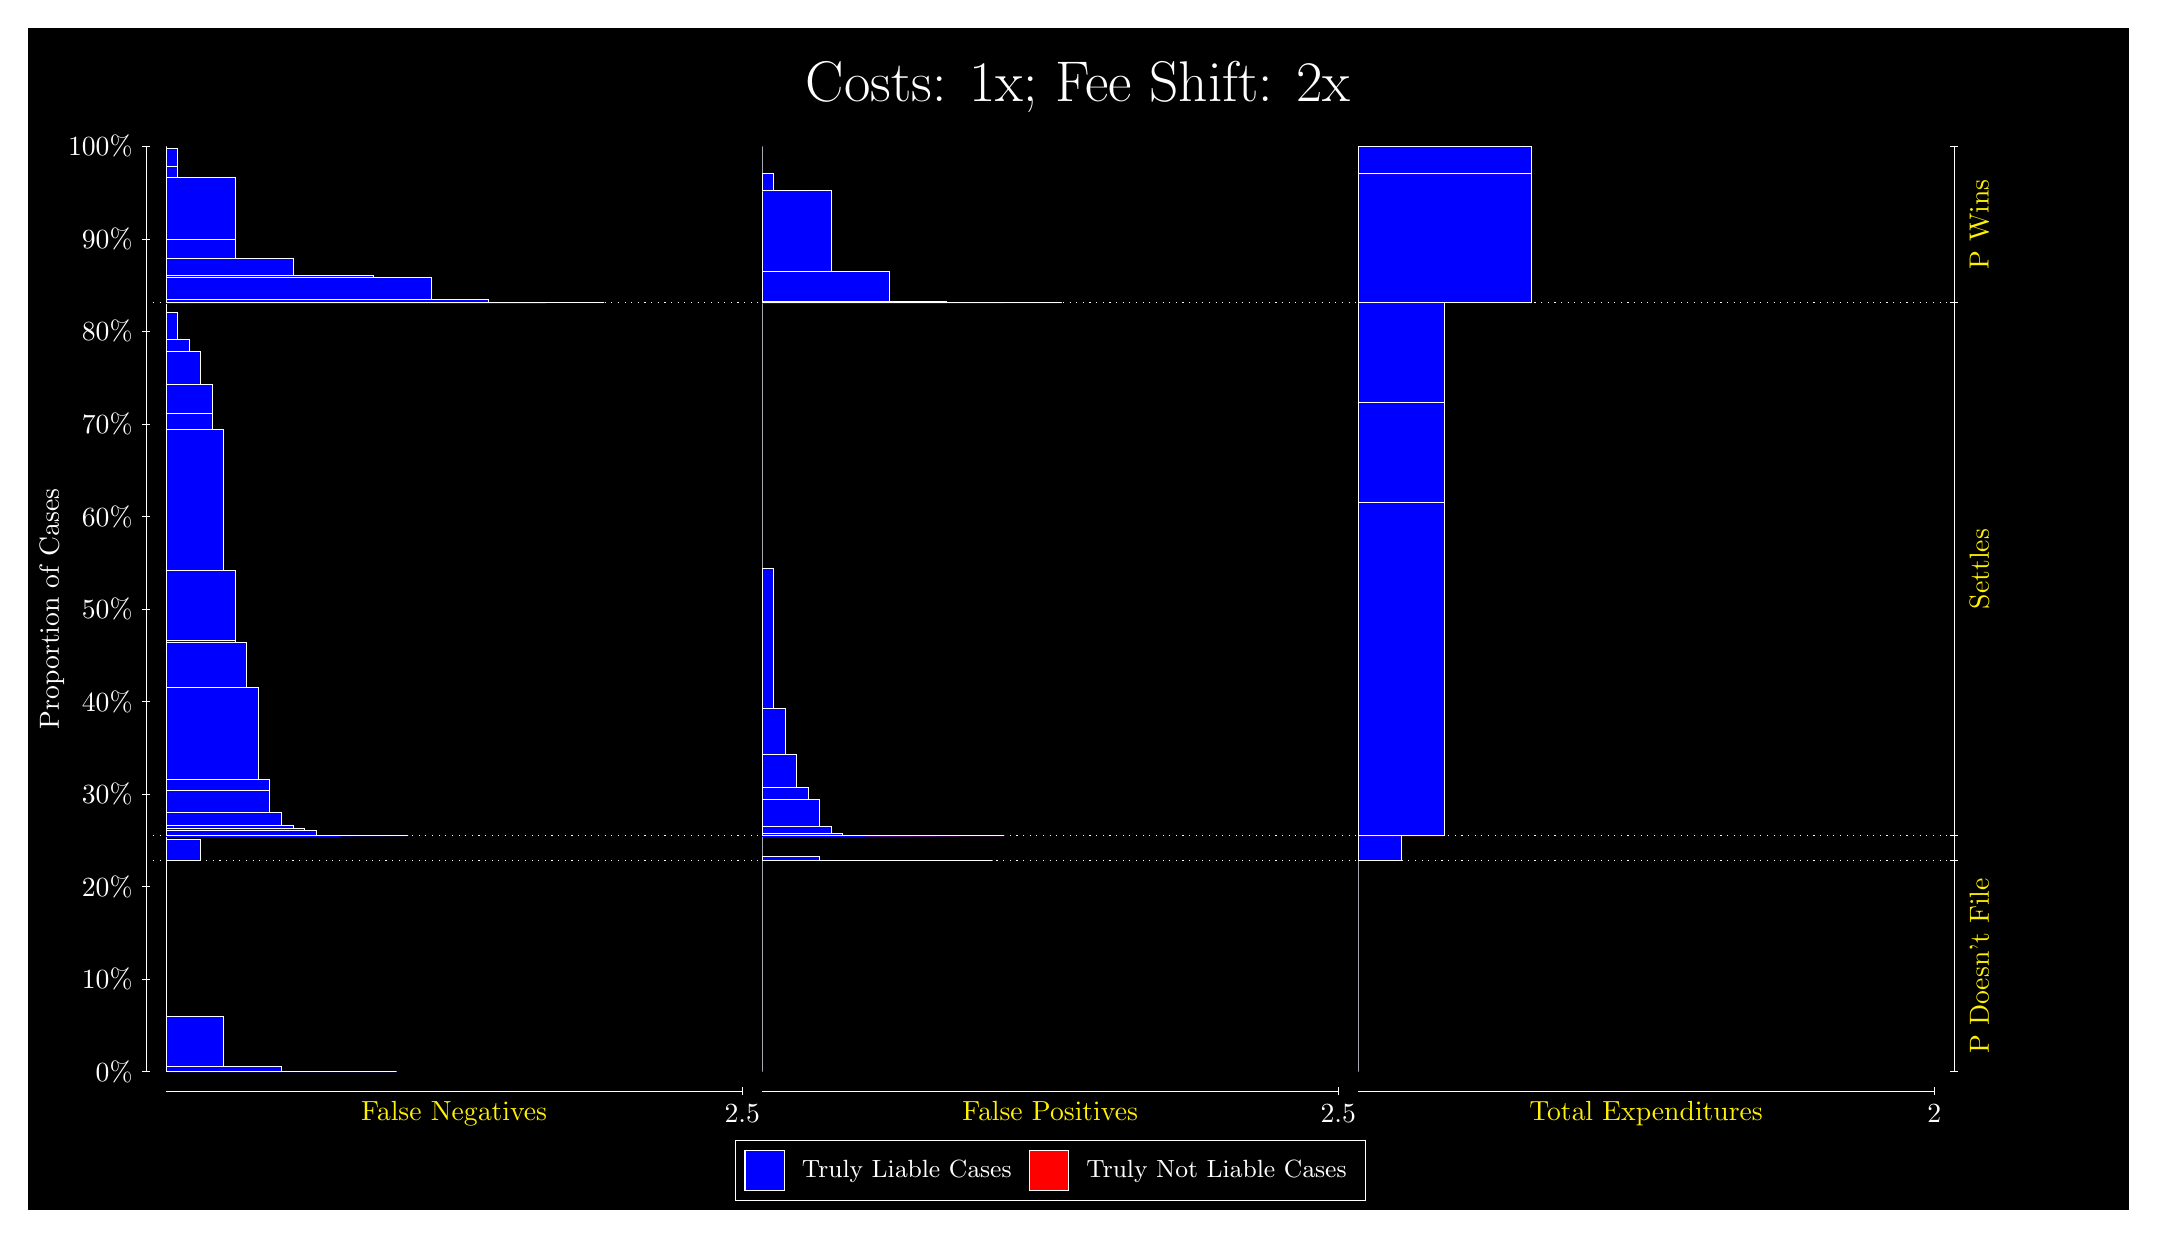
\begin{tikzpicture}
\draw[fill=black] (0,0) rectangle (26.667,15);
\draw[text=white] (0,13.5) rectangle (26.667,15) node[midway] {\huge Costs: 1x; Fee Shift: 2x};
\draw[white, very thin] (1.5,1.75) -- (1.5,13.5);
\node[rotate=90, text=white, anchor=center] at (0.3, 7.625) {Proportion of Cases};
\draw[white, very thin] (1.45,1.75) -- (1.55,1.75);
\node[text=white, anchor=east] at (1.45, 1.75) {0\%};
\draw[white, very thin] (1.45,2.925) -- (1.55,2.925);
\node[text=white, anchor=east] at (1.45, 2.925) {10\%};
\draw[white, very thin] (1.45,4.1) -- (1.55,4.1);
\node[text=white, anchor=east] at (1.45, 4.1) {20\%};
\draw[white, very thin] (1.45,5.275) -- (1.55,5.275);
\node[text=white, anchor=east] at (1.45, 5.275) {30\%};
\draw[white, very thin] (1.45,6.45) -- (1.55,6.45);
\node[text=white, anchor=east] at (1.45, 6.45) {40\%};
\draw[white, very thin] (1.45,7.625) -- (1.55,7.625);
\node[text=white, anchor=east] at (1.45, 7.625) {50\%};
\draw[white, very thin] (1.45,8.8) -- (1.55,8.8);
\node[text=white, anchor=east] at (1.45, 8.8) {60\%};
\draw[white, very thin] (1.45,9.975) -- (1.55,9.975);
\node[text=white, anchor=east] at (1.45, 9.975) {70\%};
\draw[white, very thin] (1.45,11.15) -- (1.55,11.15);
\node[text=white, anchor=east] at (1.45, 11.15) {80\%};
\draw[white, very thin] (1.45,12.325) -- (1.55,12.325);
\node[text=white, anchor=east] at (1.45, 12.325) {90\%};
\draw[white, very thin] (1.45,13.5) -- (1.55,13.5);
\node[text=white, anchor=east] at (1.45, 13.5) {100\%};

\draw[white, very thin] (24.457,1.75) -- (24.457,13.5);
\draw[white, very thin] (24.407,1.75) -- (24.507,1.75);
\node[anchor=west] at (24.407, 1.75) {};
\draw[white, very thin] (24.407,4.4326) -- (24.507,4.4326);
\node[anchor=west] at (24.407, 4.4326) {};
\draw[white, very thin] (24.407,4.746) -- (24.507,4.746);
\node[anchor=west] at (24.407, 4.746) {};
\draw[white, very thin] (24.407,11.515) -- (24.507,11.515);
\node[anchor=west] at (24.407, 11.515) {};
\draw[white, very thin] (24.407,13.5) -- (24.507,13.5);
\node[anchor=west] at (24.407, 13.5) {};

\draw[white, very thin, fill=blue] (1.75,1.75) rectangle (4.6775,1.75);
\draw[white, very thin, fill=blue] (1.75,1.75) rectangle (3.9457,1.7505);
\draw[white, very thin, fill=blue] (1.75,1.7505) rectangle (3.2138,1.8152);
\draw[white, very thin, fill=blue] (1.75,1.8152) rectangle (2.4819,2.4527);
\draw[white, very thin, fill=red] (1.75,2.4527) rectangle (1.75,2.4527);
\draw[white, very thin, fill=blue] (1.75,2.4527) rectangle (1.75,4.4326);
\draw[white, very thin, fill=blue] (1.75,4.4326) rectangle (2.1891,4.6947);
\draw[white, very thin, fill=red] (1.75,4.6947) rectangle (1.75,4.6947);
\draw[white, very thin, fill=blue] (1.75,4.6947) rectangle (1.75,4.746);
\draw[white, very thin, fill=blue] (1.75,4.746) rectangle (4.8239,4.746);
\draw[white, very thin, fill=blue] (1.75,4.746) rectangle (4.5312,4.746);
\draw[white, very thin, fill=blue] (1.75,4.746) rectangle (4.2384,4.746);
\draw[white, very thin, fill=blue] (1.75,4.746) rectangle (4.092,4.746);
\draw[white, very thin, fill=blue] (1.75,4.746) rectangle (3.9457,4.7465);
\draw[white, very thin, fill=blue] (1.75,4.7465) rectangle (3.7993,4.7467);
\draw[white, very thin, fill=blue] (1.75,4.7467) rectangle (3.6529,4.8202);
\draw[white, very thin, fill=blue] (1.75,4.8202) rectangle (3.5065,4.8432);
\draw[white, very thin, fill=blue] (1.75,4.8432) rectangle (3.3602,4.8809);
\draw[white, very thin, fill=blue] (1.75,4.8809) rectangle (3.2138,5.0468);
\draw[white, very thin, fill=blue] (1.75,5.0468) rectangle (3.0674,5.3208);
\draw[white, very thin, fill=blue] (1.75,5.3208) rectangle (3.0674,5.4598);
\draw[white, very thin, fill=blue] (1.75,5.4598) rectangle (2.921,6.6356);
\draw[white, very thin, fill=blue] (1.75,6.6356) rectangle (2.7746,7.2025);
\draw[white, very thin, fill=blue] (1.75,7.2025) rectangle (2.6283,7.2326);
\draw[white, very thin, fill=blue] (1.75,7.2326) rectangle (2.6283,8.118);
\draw[white, very thin, fill=blue] (1.75,8.118) rectangle (2.4819,9.9013);
\draw[white, very thin, fill=blue] (1.75,9.9013) rectangle (2.3355,10.115);
\draw[white, very thin, fill=blue] (1.75,10.115) rectangle (2.3355,10.483);
\draw[white, very thin, fill=blue] (1.75,10.483) rectangle (2.1891,10.901);
\draw[white, very thin, fill=blue] (1.75,10.901) rectangle (2.0428,11.048);
\draw[white, very thin, fill=blue] (1.75,11.048) rectangle (1.8964,11.049);
\draw[white, very thin, fill=blue] (1.75,11.049) rectangle (1.8964,11.397);
\draw[white, very thin, fill=red] (1.75,11.397) rectangle (1.75,11.397);
\draw[white, very thin, fill=blue] (1.75,11.397) rectangle (1.75,11.515);
\draw[white, very thin, fill=blue] (1.75,11.515) rectangle (7.3123,11.515);
\draw[white, very thin, fill=blue] (1.75,11.515) rectangle (6.5805,11.516);
\draw[white, very thin, fill=blue] (1.75,11.516) rectangle (5.8486,11.557);
\draw[white, very thin, fill=blue] (1.75,11.557) rectangle (5.1167,11.831);
\draw[white, very thin, fill=blue] (1.75,11.831) rectangle (4.8239,11.831);
\draw[white, very thin, fill=blue] (1.75,11.831) rectangle (4.3848,11.864);
\draw[white, very thin, fill=blue] (1.75,11.864) rectangle (4.092,11.864);
\draw[white, very thin, fill=blue] (1.75,11.864) rectangle (3.6529,11.864);
\draw[white, very thin, fill=blue] (1.75,11.864) rectangle (3.3602,12.078);
\draw[white, very thin, fill=blue] (1.75,12.078) rectangle (2.921,12.078);
\draw[white, very thin, fill=blue] (1.75,12.078) rectangle (2.6283,12.323);
\draw[white, very thin, fill=blue] (1.75,12.323) rectangle (2.6283,13.101);
\draw[white, very thin, fill=blue] (1.75,13.101) rectangle (1.8964,13.246);
\draw[white, very thin, fill=blue] (1.75,13.246) rectangle (1.8964,13.477);
\draw[white, very thin, fill=red] (1.75,13.477) rectangle (1.75,13.477);
\draw[white, very thin, fill=blue] (1.75,13.477) rectangle (1.75,13.5);
\draw[white, very thin, fill=red] (9.3189,1.75) rectangle (9.3189,1.75);
\draw[white, very thin, fill=blue] (9.3189,1.75) rectangle (9.3189,4.4326);
\draw[white, very thin, fill=red] (9.3189,4.4326) rectangle (12.246,4.4326);
\draw[white, very thin, fill=blue] (9.3189,4.4326) rectangle (12.246,4.4326);
\draw[white, very thin, fill=blue] (9.3189,4.4326) rectangle (11.515,4.4326);
\draw[white, very thin, fill=blue] (9.3189,4.4326) rectangle (10.783,4.4331);
\draw[white, very thin, fill=blue] (9.3189,4.4331) rectangle (10.051,4.4839);
\draw[white, very thin, fill=blue] (9.3189,4.4839) rectangle (9.3189,4.746);
\draw[white, very thin, fill=red] (9.3189,4.746) rectangle (12.393,4.746);
\draw[white, very thin, fill=blue] (9.3189,4.746) rectangle (12.393,4.746);
\draw[white, very thin, fill=red] (9.3189,4.746) rectangle (11.807,4.746);
\draw[white, very thin, fill=blue] (9.3189,4.746) rectangle (11.807,4.746);
\draw[white, very thin, fill=blue] (9.3189,4.746) rectangle (11.661,4.746);
\draw[white, very thin, fill=red] (9.3189,4.746) rectangle (11.515,4.746);
\draw[white, very thin, fill=blue] (9.3189,4.746) rectangle (11.515,4.746);
\draw[white, very thin, fill=red] (9.3189,4.746) rectangle (11.222,4.746);
\draw[white, very thin, fill=blue] (9.3189,4.746) rectangle (11.222,4.746);
\draw[white, very thin, fill=blue] (9.3189,4.746) rectangle (11.075,4.746);
\draw[white, very thin, fill=red] (9.3189,4.746) rectangle (10.929,4.746);
\draw[white, very thin, fill=blue] (9.3189,4.746) rectangle (10.929,4.7461);
\draw[white, very thin, fill=blue] (9.3189,4.7461) rectangle (10.783,4.7461);
\draw[white, very thin, fill=red] (9.3189,4.7461) rectangle (10.636,4.7461);
\draw[white, very thin, fill=blue] (9.3189,4.7461) rectangle (10.636,4.7464);
\draw[white, very thin, fill=blue] (9.3189,4.7464) rectangle (10.49,4.7561);
\draw[white, very thin, fill=red] (9.3189,4.7561) rectangle (10.344,4.7561);
\draw[white, very thin, fill=blue] (9.3189,4.7561) rectangle (10.344,4.7757);
\draw[white, very thin, fill=blue] (9.3189,4.7757) rectangle (10.197,4.8647);
\draw[white, very thin, fill=red] (9.3189,4.8647) rectangle (10.051,4.8647);
\draw[white, very thin, fill=blue] (9.3189,4.8647) rectangle (10.051,5.2135);
\draw[white, very thin, fill=blue] (9.3189,5.2135) rectangle (9.9044,5.3607);
\draw[white, very thin, fill=blue] (9.3189,5.3607) rectangle (9.758,5.7785);
\draw[white, very thin, fill=blue] (9.3189,5.7785) rectangle (9.6116,6.3601);
\draw[white, very thin, fill=blue] (9.3189,6.3601) rectangle (9.4652,8.1434);
\draw[white, very thin, fill=blue] (9.3189,8.1434) rectangle (9.3189,11.515);
\draw[white, very thin, fill=red] (9.3189,11.515) rectangle (13.125,11.515);
\draw[white, very thin, fill=blue] (9.3189,11.515) rectangle (13.125,11.515);
\draw[white, very thin, fill=red] (9.3189,11.515) rectangle (12.393,11.515);
\draw[white, very thin, fill=blue] (9.3189,11.515) rectangle (12.393,11.515);
\draw[white, very thin, fill=red] (9.3189,11.515) rectangle (11.661,11.515);
\draw[white, very thin, fill=blue] (9.3189,11.515) rectangle (11.661,11.538);
\draw[white, very thin, fill=red] (9.3189,11.538) rectangle (10.929,11.538);
\draw[white, very thin, fill=blue] (9.3189,11.538) rectangle (10.929,11.914);
\draw[white, very thin, fill=blue] (9.3189,11.914) rectangle (10.197,12.937);
\draw[white, very thin, fill=red] (9.3189,12.937) rectangle (9.9044,12.937);
\draw[white, very thin, fill=blue] (9.3189,12.937) rectangle (9.9044,12.937);
\draw[white, very thin, fill=blue] (9.3189,12.937) rectangle (9.4652,13.152);
\draw[white, very thin, fill=red] (9.3189,13.152) rectangle (9.3189,13.152);
\draw[white, very thin, fill=blue] (9.3189,13.152) rectangle (9.3189,13.5);
\draw[white, very thin, fill=red] (16.888,1.75) rectangle (16.888,1.75);
\draw[white, very thin, fill=blue] (16.888,1.75) rectangle (16.888,4.4326);
\draw[white, very thin, fill=red] (16.888,4.4326) rectangle (17.437,4.4326);
\draw[white, very thin, fill=blue] (16.888,4.4326) rectangle (17.437,4.746);
\draw[white, very thin, fill=red] (16.888,4.746) rectangle (17.986,4.746);
\draw[white, very thin, fill=blue] (16.888,4.746) rectangle (17.986,8.9835);
\draw[white, very thin, fill=red] (16.888,8.9835) rectangle (17.986,8.9835);
\draw[white, very thin, fill=blue] (16.888,8.9835) rectangle (17.986,10.253);
\draw[white, very thin, fill=red] (16.888,10.253) rectangle (17.986,10.253);
\draw[white, very thin, fill=blue] (16.888,10.253) rectangle (17.986,11.515);
\draw[white, very thin, fill=red] (16.888,11.515) rectangle (19.083,11.515);
\draw[white, very thin, fill=blue] (16.888,11.515) rectangle (19.083,13.152);
\draw[white, very thin, fill=red] (16.888,13.152) rectangle (19.083,13.152);
\draw[white, very thin, fill=blue] (16.888,13.152) rectangle (19.083,13.5);
\draw[white, dotted] (1.5,4.4326) -- (24.457,4.4326);
\draw[white, dotted] (1.5,4.746) -- (24.457,4.746);
\draw[white, dotted] (1.5,11.515) -- (24.457,11.515);
\draw[white, very thin] (1.75,1.5) -- (9.0689,1.5);
\node[text=yellow, anchor=north] at (5.4094, 1.5) {False Negatives};
\draw[white, very thin] (9.0689,1.45) -- (9.0689,1.55);
\node[text=white, anchor=north] at (9.0689, 1.45) {2.5};

\draw[white, very thin] (9.3189,1.5) -- (16.638,1.5);
\node[text=yellow, anchor=north] at (12.978, 1.5) {False Positives};
\draw[white, very thin] (16.638,1.45) -- (16.638,1.55);
\node[text=white, anchor=north] at (16.638, 1.45) {2.5};

\draw[white, very thin] (16.888,1.5) -- (24.207,1.5);
\node[text=yellow, anchor=north] at (20.547, 1.5) {Total Expenditures};
\draw[white, very thin] (24.207,1.45) -- (24.207,1.55);
\node[text=white, anchor=north] at (24.207, 1.45) {2};

\node[text=yellow, centered, rotate=90] at (24.777, 3.0913) {P Doesn't File};

\node[text=yellow, centered, rotate=90] at (24.777, 8.1307) {Settles};
\node[text=yellow, centered, rotate=90] at (24.777, 12.508) {P Wins};

\draw (12.978300999999998,1.5) node[draw=none] (baseCoordinate) {};
\begin{scope}[align=center]
        \matrix[scale=0.5, draw=white, below=0.5cm of baseCoordinate, nodes={draw}, column sep=0.1cm]{
            \node[rectangle, draw, minimum width=0.5cm, minimum height=0.5cm, fill=blue] {}; &
            \node[draw=none, font=\small, text=white] (B) {Truly Liable Cases}; &
            \node[rectangle, draw, minimum width=0.5cm, minimum height=0.5cm, fill=red] {}; &
            \node[draw=none, font=\small, text=white] (B) {Truly Not Liable Cases}; \\
            };
\end{scope}

\end{tikzpicture}
\end{document}